Sei \(\mathcal{M}^{2k}\) eine \((k-1)\)-zusammenh\"angende \(\pi\)-Mannigfaltigkeit mit \(k\geq3\), deren Rand entweder leer oder eine Homotopiesph\"are ist. Um \(\mathcal{M}\) durch Chirurgie in eine \(k\)-zusammenh\"angende \(\pi\)-Mannigfaltigkeit zu \"uberf\"uhren m\"ussen einige Hindernisse beachtet werden. Einerseits muss das Normalenb\"undel einer eingebetteten \(k\)-Sph\"are nicht unbedingt trivial sein, andererseits ist nicht jede Sph\"are primitiv und vereinfacht somit nicht unbedingt die Homologie. In diesem Fall ist die mittlere Homologiegruppe \(H_k(\mathcal{M})\) jedoch frei, sodass keine Komplikationen durch Torsion auftreten. 
\begin{lemma}\label{lem:middle_free}
    Sei \(\mathcal{M}^{2k}\) mit \({H_k(\partial\mathcal{M})=H_{k-1}(\partial\mathcal{M})=0}\) derart, dass \(H_{k-1}(\mathcal{M})\) frei ist. Dann ist auch \(H_k(\mathcal{M})\) frei.
\end{lemma}
\begin{proof}
    Aus der Annahme an den Rand folgt, dass \(q^*\colon H_k(\mathcal{M})\to H_k(\mathcal{M},\partial\mathcal{M})\) ein Isomorphismus ist. Sei \(T_k\) die Torsionsuntergruppe von \(H_k(\mathcal{M})\). Es folgt
    \[H_k(\mathcal{M})\mathop{\cong}^{q^*}H_k(\mathcal{M},\partial\mathcal{M})\overcong{P.D.}H^k(\mathcal{M})\overcong{U.K.}\operatorname{Hom}(H_k(\mathcal{M}),\mathbb{Z})\cong H_k(\mathcal{M})/T_k\,.\]
    Somit muss \(T_k=0\), und \(H_k(\mathcal{M})\) frei sein.
\end{proof}

\subsection{Repr\"asentierende Sph\"aren}
    Sei \(\mathcal{M}^{2k}\) eine \((k-1)\)-zusammenh\"angende \(\pi\)-Mannigfaltigkeit und \(x\in H_k(\mathcal{M})\). Gem\"a\ss{} dem Satz von Hurewicz ist
    \[h\colon\pi_k(\mathcal{M})\to H_k(\mathcal{M}),\,\eqcl{\gamma}\mapsto\gamma_*\big(\eqcl{\mathbb{S}^k}\big)\]
    ein Isomorphimus. Es existiert also eine bis auf Homotopie eindeutig bestimmte Funktion \(\phi\colon\mathbb{S}^k\to\mathcal{M}\) mit \(\phi_*\eqcl{\mathbb{S}^k}=x\). Aufgrund eines Satzes von Haelfiger (\cite{haefliger1961differentiable} Satz 1) kann f\"ur \(k\geq3\) angenommen werden dass \(\phi\) eine Einbettung ist. Bezeichne die eingebettete Sph\"are durch \(\mathcal{S}(x)\). Diese ist f\"ur \(k\geq4\) bis auf Isotopie eindeutig bestimmt, sodass sich die Homotopieklasse der Kupplungsfunktion des Normalenb\"undels von \(\mathcal{S}(x)\) in \(\mathcal{M}\) betrachten l\"asst. F\"ur \(k\geq4\) ist also die Funktion
    \[\alpha\colon H_k(\mathcal{M})\to\pi_{k-1}(\operatorname{SO}(k)),\,x\mapsto\eqcl{\nu(\mathcal{S}(x))}\]
    wohldefiniert. Aufgrund von \(\pi_2(\operatorname{SO}(3))=0\) l\"asst sich \(\alpha\) auch f\"ur \(k=3\) definieren. Es folgt nun aus vorherigen \"Uberlegungen \ref{subsec:stable_normal_bundle}, das \(\alpha(x)\) ein ganzzahliges Vielfaches der Kupplungsfunktion des Normalenb\"undels ist, und
    \begin{equation}\label{eq:alpha_kernel}
        \alpha(x)\in\ker S_*\cong\begin{cases}
            \mathbb{Z} & k=2m\\
            \mathbb{Z}_2 & k=2m+1\notin\{3,7\}\\
            0 & k\in\{3,7\}
        \end{cases}
    \end{equation}
    gilt. Die Entscheidung, wann das Normalenb\"undel trivial ist, h\"angt also von der Parit\"at von \(k\) ab.

\subsection{Symplektische Basen}
    \begin{definition}[Schwach symplektische Basis]
        Sei \(M^{2k}\) ein freier \(R\)-Modul. Eine Basis \((e_i,f_i)_{1\leq i\leq k}\) von \(M\), hei\ss e schwach symplektisch bez\"uglich einer Bilinearform \(\beta\colon M\otimes M\to R\), falls
        \[\beta(e_i,f_j)=\delta_{ij}\quad\text{und}\quad\beta(e_i,e_j)=\beta(f_i,f_j)=0\quad\text{f\"ur alle}\quad1\leq i,j\leq k\,.\]
    \end{definition}
    Ist \(\beta\) schiefsymmetrisch, hei\ss e sie symplektisch. Die Signifikanz dieser Basen liegt unter anderem in folgendem Satz.
    \begin{theorem}\label{thm:even_symp_ann}
        Sei \(k\geq3\) und \(\mathcal{M}^{2k}\) eine \((k-1)\)-zusammenh\"angende, gerahmte Mannigfaltigkeit, deren Rand leer oder eine Homotopiesph\"are ist, sodass \(H_k(\mathcal{M})\) eine schwach symplektische Basis \(e_i,f_i\) mit \(\alpha(e_i)=0\) besitzt. Dann kann \(H_k(\mathcal{M})\) durch gerahmte Chirurgie vernichtet werden.
    \end{theorem}
    \begin{proof}
        Da \(e_1\) ein triviales Normalenb\"undel besitzt, kann Chirurgie an \(e_1\) durchgef\"uhrt werden. Sei \(\mathcal{S}\) die Anklebesph\"are und \(\mathcal{M}^{\prime}\) die resultierende Mannigfaltigkeit. Da die \(e_i,f_i\) eine schwach symplektische Basis bilden, ist \(e_1\) primitiv, und es gilt f\"ur
        \[\phi\colon H_i(\mathcal{M})\to\mathbb{Z},\,x\mapsto x\cdot e_1\]
        gerade \(\ker\phi=H_i(\mathcal{M})/\langle f_1\rangle\). Aus Satz \ref{lem:even_surg_effect} folgt
        \[H_i(\mathcal{M}^{\prime})\cong\ker\phi/\langle e_1\rangle\cong H_i(\mathcal{M})/\langle e_1,f_1\rangle\,.\]
        \"Uber Transversalit\"at kann angenommen werden, dass die Bilder \(e_i^{\prime},f_i^{\prime}\in H_i(\mathcal{M}^{\prime})\) durch Sph\"aren in \(\mathcal{M}\setminus\mathcal{S}\) repr\"asentiert werden, sodass sich die Schnittzahlen nicht \"andern und die \(e_i^{\prime},f_i^{\prime}\) erneut eine symplektische Basis mit \(\alpha(e_i^{\prime})=0\) bilden. Die Aussage folgt rekursiv.
    \end{proof}
    Es wird im Folgenden noch eine weitere symplektische Basis \({e_i,f_i\in H_k(\partial\mathcal{W})}\) ben\"otigt werden, wobei alle \(e_i\) im Kern der Inklusion \({\partial\mathcal{W}\hookrightarrow\mathcal{W}^{2k+1}}\) liegen. Hierbei sei stets an den Torus erinnert. Es gilt \({H_1(\mathbb{S}^1\times\mathbb{S}^1)\cong\mathbb{Z}\oplus\mathbb{Z}}\), wobei die Erzeuger eine symplektische Basis bilden. Eines der Elemente liegt im Kern der Inklusion \(\mathbb{S}^1\times\mathbb{S}^1\hookrightarrow\mathbb{D}^2\times\mathbb{S}^1\) des Torus als Rand des Volltorus. Es wird folgendes Lemma ben\"otigt. Im folgenden Satz bezeichne \(\operatorname{Ad}\) zu einem K\"orper \(\mathbb{K}\) die Abbildung
    \[\operatorname{Ad}\colon H_i(\partial\mathcal{W};\mathbb{K})\to\operatorname{Hom}(H_{n-i}(\partial\mathcal{W};\mathbb{K}),\mathbb{K}),\,x\mapsto x\cdot(\mathrel{-})\,.\]
    \begin{lemma}\label{lem:inter_annihilates}
        Sei \(\mathbb{K}\) ein K\"orper, \(\mathcal{W}^{2k+1}\) eine Mannigfaltigkeit, 
        \[A_i:=\ker\left(\iota_*\colon H_i(\partial\mathcal{W};\mathbb{K})\to H_i(\mathcal{W};\mathbb{K})\right)\]
        und \(R\colon\operatorname{Hom}(H_{n-i}(\partial\mathcal{W};\mathbb{K}),\mathbb{K})\to\operatorname{Hom}(A_{n-i},\mathbb{K})\) die Einschr\"ankung, dann ist der Kern von \(F:=R\circ\operatorname{Ad}\) gerade \(A_i\).
    \end{lemma}
    \begin{proof}
        Ein \(x\in H_i(\partial\mathcal{W};\mathbb{K})\) liegt genau dann in \(\ker F\), wenn \({(A_{n-i})\cdot x=0}\) ist. Betrachte das bis auf Vorzeichen kommutive Diagramm
        \begin{center}
            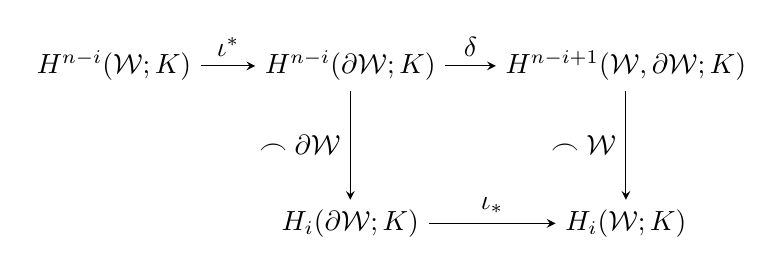
\begin{tikzpicture}
                \draw 
                    (-3, 0) node (A) {\(H^{n-i}(\mathcal{W};\mathbb{K})\)}
                    (0, 0) node (B) {\(H^{n-i}(\partial\mathcal{W};\mathbb{K})\)}
                    (3.5, 0) node (C) {\(H^{n-i+1}(\mathcal{W},\partial\mathcal{W};\mathbb{K})\)}
                    (0, -2) node (E) {\(H_i(\partial\mathcal{W};\mathbb{K})\)}
                    (3.5, -2) node (F) {\(H_i(\mathcal{W};\mathbb{K})\)}

                    (A) edge [-stealth] node [above] {\(\iota^*\)} (B)
                    (B) edge [-stealth] node [above] {\(\delta\)} (C)
                    (B) edge [-stealth] node [left] {\(\frown\eqcl{\partial\mathcal{W}}\)} (E)
                    (C) edge [-stealth] node [left] {\(\frown\eqcl{\mathcal{W}}\)} (F)
                    (E) edge [-stealth] node [above] {\(\iota_*\)} (F)
                    ;
            \end{tikzpicture}
        \end{center}
        F\"ur \(x\in H_i(\partial\mathcal{W};\mathbb{K})\) gilt
        \[(A_{n-i})\cdot x=\langle(\ker\iota_*)^*,x\rangle=\langle\im\iota^*,x\rangle=\langle H^{n-i}(\mathcal{W};\mathbb{K}),\iota_*x\rangle\,.\]
        Also liegt \(x\) genau dann im Kern von \(F\), wenn \(\langle H^{n-i}(\mathcal{W};\mathbb{K}),\iota_*x\rangle=0\) ist. Da \(\mathbb{K}\) ein K\"orper und die Kronecker-Paarung nicht degeneriert ist, ist dies zu \(x\in\ker\iota_*=A_i\) \"aquivalent.
    \end{proof}
    Die Beweisidee entstammt hierbei \cite{tomdieck2008algebraic} Proposition 18.7.5. Es ergibt sich somit \(\dim_{\mathbb{K}}A_{n-i}=\dim_{\mathbb{K}}H_i(\partial\mathcal{W};\mathbb{K})-\dim_{\mathbb{K}}A_i\), insbesondere also
    \begin{equation}\label{eq:ker_incl_dim}
        \dim_{\mathbb{K}}H_k(\partial\mathcal{W};\mathbb{K})=2\dim_{\mathbb{K}}A_k=2\dim_{\mathbb{K}}\ker\iota_*\,.
    \end{equation}
    Beachte, dass die Forderung, dass \(\mathbb{K}\) ein K\"orper n\"otig ist, da \(H_k(\mathcal{W})\) Torsion aufweisen k\"onnte. In diesem Fall k\"onnte die Kronecker-Paarung degeneriert sein. Wird Torsion herausgeteilt, gilt der vorherige Satz auch f\"ur \(\mathbb{Z}\)-Koeffizienten. Siehe etwa \cite{hatcher2002algebraic} Proposition 3.38. F\"ur die Abbildung
    \[\iota_*^{\prime}\colon H_k(\partial\mathcal{W})\xrightarrow{\iota_*}H_k(\mathcal{W})\xrightarrow{p}H_k(\mathcal{W})/T_k(\mathcal{W})\]
    gilt also gerade \(2\operatorname{Rang}\ker\iota_*^{\prime}=\operatorname{Rang}H_k(\partial\mathcal{W})\). Da das Herausteilen der Torsion keinen Einfluss auf den Rang hat, gilt \(\operatorname{Rang}\ker\iota_*=\operatorname{Rang}\ker\iota_*^{\prime}\) und
    \begin{equation}
        \operatorname{Rang}H_k(\partial\mathcal{W})=2\operatorname{Rang}\ker\iota_*\,.
    \end{equation}

    \begin{theorem}\label{thm:symp_base_ann}
        Sei \(k\) ungerade und \(\mathcal{M}^{2k}\) eine Mannigfaltigkeit mit \(H_k(\partial\mathcal{M})=H_{k-1}(\partial\mathcal{M})=0\). Dann existiert eine symplektische Basis von \(H_k(\mathcal{M})\) mit \(e_i\in\ker\iota_*\).
    \end{theorem}
    \begin{proof}
        Da \(k\) ungerade ist, besitzt \(H_k(\mathcal{M})\) geraden Rang, und es gilt \(x\cdot x=0\) f\"ur alle \(x\in H_k(\mathcal{M})\). Sei \(e_1\in\ker\iota_*\). Da die Schnittform unimodular ist, existiert ein \(f_1\in H_k(\mathcal{M})\) mit \(e_1\cdot f_1=1\). Da die Schnittform unimodular ist, spaltet \(f_i\) von \(H_k(\mathcal{M})\) und \(e_i\) von \(\ker\iota_*\) ab, sodass die Aussage rekursiv folgt.
    \end{proof}